%!TEX root = ../hbrs-poster.tex
\documentclass[hbrs-poster.tex]{subfiles}
\usepackage{hyperref}
\usepackage{xcolor}

\begin{document}
    \block{Introduction}
    {

        \textbf{Project Overview:}

        Movie genre classification plays a crucial role in content recommendation systems by providing personalized movie suggestions, boosting user engagement. It significantly improves search functionality, allowing for efficient genre-based filtering and accurate search results. 

        A genre classifier is developed that identifies the various genres a movie falls under given the plot summary.

        This provides valuable insights into audience preferences and market trends. This information is crucial for content producers and marketers to understand genre popularity to make decisions about future content creation and marketing strategies.\\
        % This classification also facilitates content analysis and insights, enabling trend analysis and guiding market research for informed content production and marketing decisions. Additionally, it supports content creation by helping creators align with genre norms and audience expectations, while also aiding in the curation of thematic or genre-specific collections to improve user experience 
        \textbf{Dataset:}
        \begin{itemize}
            \item 42,306 movie plot summaries extracted from IMDB and Wikipedia, with 362 different genres. 
            \item \textbf{Note:} Multi-label classification of movies by genre is challenging due to several reasons that might be contributing to the low performance. Some of these challenges include:
            \begin{itemize}
                \item Movie genres often have complex relationships and overlaps, making it difficult for models to distinguish between them based solely on features. We visualized the correlation between various genres, maintaining the genres with reasonable amount of overlapping with other labels to improve the performance.
                \begin{tikzfigure}
                    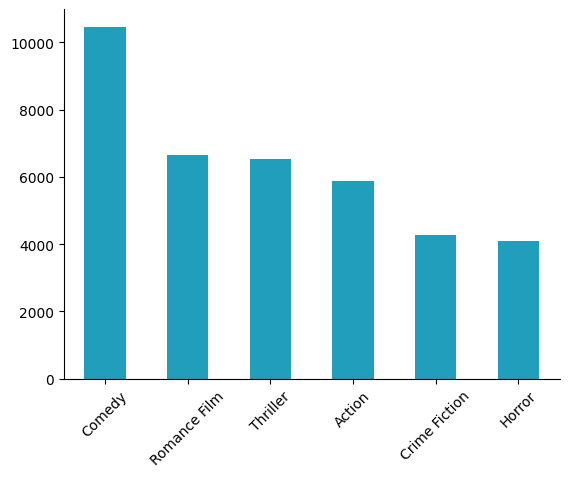
\includegraphics[width=0.18\textwidth, height=0.10\textheight]{figures/output2.png}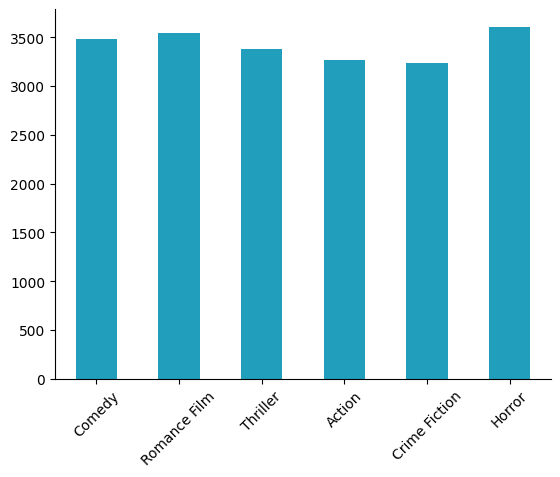
\includegraphics[width=0.18\textwidth, height=0.10\textheight]{figures/output3.png}
                \end{tikzfigure}
                \item The imbalance in movies dataset can cause the model to be biased towards the more frequent genres. We remove few-shot labels at the first step, and perform statistical sampling from the original dataset to prevent biased results from trained model.
                
                
            \end{itemize}      
        \end{itemize}   
    }
\end{document}
